% Stereographic and cylindrical map projections
% Author: Tomasz M. Trzeciak
% Source: LaTeX-Community.org
%         <http://www.latex-community.org/viewtopic.php?f=4&t=2111>

% Need fig_gps_3d_preamb_01.tex

\newcommand\pgfmathsinandcos[3]{%
  \pgfmathsetmacro#1{sin(#3)}%
  \pgfmathsetmacro#2{cos(#3)}%
}
\newcommand\LongitudePlane[3][current plane]{%
  \pgfmathsinandcos\sinEl\cosEl{#2} % elevation
  \pgfmathsinandcos\sint\cost{#3} % azimuth
  \tikzset{#1/.style={cm={\cost,\sint*\sinEl,0,\cosEl,(0,0)}}}
}
\newcommand\LatitudePlane[3][current plane]{%
  \pgfmathsinandcos\sinEl\cosEl{#2} % elevation
  \pgfmathsinandcos\sint\cost{#3} % latitude
  \pgfmathsetmacro\yshift{\cosEl*\sint}
  \tikzset{#1/.style={cm={\cost,0,0,\cost*\sinEl,(0,\yshift)}}} %
}
\newcommand\DrawLongitudeCircle[2][1]{
  \LongitudePlane{\angEl}{#2}
  \tikzset{current plane/.prefix style={scale=#1}}
   % angle of "visibility"
  \pgfmathsetmacro\angVis{atan(sin(#2)*cos(\angEl)/sin(\angEl))} %
  \draw[current plane] (\angVis:1) arc (\angVis:\angVis+180:1);
  \draw[current plane,dashed] (\angVis-180:1) arc (\angVis-180:\angVis:1);
}
\newcommand\DrawLatitudeCircle[2][1]{
  \LatitudePlane{\angEl}{#2}
  \tikzset{current plane/.prefix style={scale=#1}}
  \pgfmathsetmacro\sinVis{sin(#2)/cos(#2)*sin(\angEl)/cos(\angEl)}
  % angle of "visibility"
  \pgfmathsetmacro\angVis{asin(min(1,max(\sinVis,-1)))}
  \draw[current plane] (\angVis:1) arc (\angVis:-\angVis-180:1);
  \draw[current plane,dashed] (180-\angVis:1) arc (180-\angVis:\angVis:1);
}

% Latitude-longitude
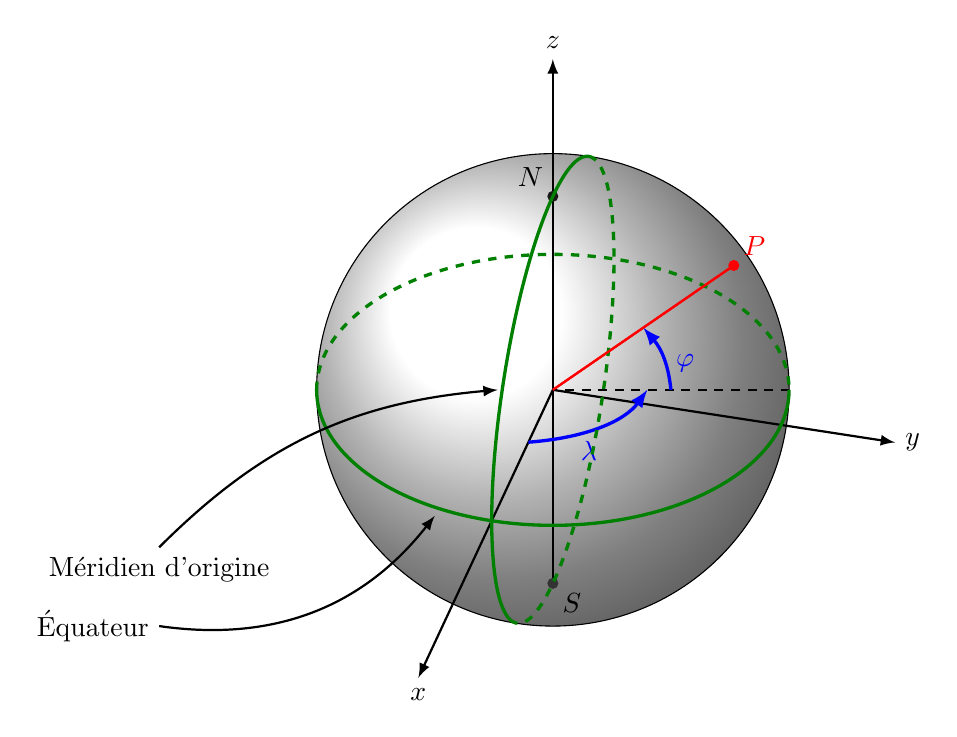
\begin{tikzpicture}[scale=1]
%% some definitions

\def\R{3} % sphere radius
\def\angEl{35} % elevation angle
\def\angAz{-105} % azimuth angle
\def\angPhi{0} % longitude of point P
\def\angBeta{40} % latitude of point P

%% working planes

\pgfmathsetmacro\H{\R*cos(\angEl)} % distance to north pole
\tikzset{xyplane/.style={cm={cos(\angAz),sin(\angAz)*sin(\angEl),-sin(\angAz),
                              cos(\angAz)*sin(\angEl),(0,0)}}}
\LongitudePlane[xzplane]{\angEl}{\angAz}
\LongitudePlane[pzplane]{\angEl}{\angPhi}
\LatitudePlane[equator]{\angEl}{0}

%% draw xyplane and sphere

%\draw[xyplane] (-2*\R,-2*\R) rectangle (2.2*\R,2.8*\R);
\fill[ball color=white] (0,0) circle (\R); % 3D lighting effect
\draw (0,0) circle (\R);

%% characteristic points

\coordinate (O) at (0,0);
\coordinate (N) at (0,\H);
\coordinate (S) at (0,-\H);
\path[pzplane] (\angBeta:\R) coordinate (P);
\path[pzplane] (\R,0) coordinate (PE);
\path[xzplane] (\R,0) coordinate (XE);
\path (PE) ++(0,-\H) coordinate (Paux); % to aid Phat calculation
\coordinate (Phat) at (intersection cs: first line={(N)--(P)},
                                        second line={(S)--(Paux)});

%% draw xyz coordinate system

\draw[xyplane,<->,>=latex, thick] (2.2*\R,0) node[below] {$x$} -- (0,0) -- (0,1.5*\R)
    node[right] {$y$};
\draw[->,>=latex, thick] (0,-\H) -- (0,1.4*\R) node[above] {$z$};

%% draw lines and put labels

%\draw[dashed] (P) -- (N) +(0.3ex,0.6ex) node[above left] {$N$};
\fill[black!90] (N) circle (2pt) node[above left, black] {$N$};
\fill[black!80] (S) circle (2pt) node[below right, black] {$S$};
%\draw (P) -- (Phat) node[above right] {$\mathbf{\hat{P}}$};
\draw[thick, red] (O) -- (P);
\fill[red] (P) circle (2pt) node[above right] {$P$};
\draw[dashed, thick] (XE) -- (O) -- (PE);
\draw[pzplane,>=latex,->,very thick,blue] (0:0.5*\R) to[bend right=15]
    node[pos=0.4,right] {$\varphi$} (\angBeta:0.5*\R);
\draw[equator,>=latex,->,very thick,blue] (\angAz:0.4*\R) to[bend right=30]
    node[pos=0.4,below] {$\lambda$} (\angPhi:0.4*\R);

%% draw meridians and latitude circles

 \DrawLatitudeCircle[\R,green!50!black, very thick]{0} % equator
 \DrawLongitudeCircle[\R,green!50!black, very thick]{\angAz} % xzplane
 \draw[thick, red] (O) -- (P);
 
\draw[->,>=latex,thick,black] (-5,-3) node[left] {\'Equateur} 
to [bend right=30] (-1.5,-1.6); 

\draw[->,>=latex,thick,black] (-5,-2) node[below] {M\'eridien d'origine} 
to [bend left=20] (-0.7,0);
\end{tikzpicture}